%
\providecommand{\main}{../..}
\documentclass[../../main.tex]{subfiles}
\begin{document}

\chapter{Entropy and the Emergence of Time}
\lesson{14}{8/4/20}

\textbf{Irreversibility} is one of the fundamental aspects of reality as we know it. It describes why it is easy for things to break, scatter or decay, and why it is hard --- or in certain cases impossible --- to return them to their previous unscathed state. Irreversible processes are a key indicator of the \textit{directionality} of time, physical remainders of the difference between the past we remember and the future we try to predict.

\medskip

Statistical Mechanics allows us to understand --- at least in part --- why irreversibility exists, and where does it come from. In that regard, we will start our discussion by stating two important results: Liouville's theorem and the Poincaré Recurrence theorem. 

\medskip

The first deals with the evolution of ensembles, showing that patches of phase-space \textit{flow} like incompressible fluids. This will provide both a stochastic origin of irreversibility and also a more convincing motivation for the microcanonical equiprobability postulate.

\medskip

On the other hand, the Poincaré recurrence theorem will reveal the illusory nature of irreversibility, as given sufficient time everything can be reversed. However, Poincaré recurrence works on \textit{unfathomably long} time scales --- completely hiding its effects from our experience. 

\medskip
 
When talking about irreversibility, it is almost impossible not to include \textbf{entropy}, and the consequences of the \textit{second law of thermodynamics}. After revising the two different definitions we gave of $S$ --- the one from classical thermodynamics, and the other from Statistical Mechanics --- we will introduce a \textit{third} point of view, originating from \textbf{information theory}, which will prove extremely useful, allowing us to re-derive the entire equilibrium statistical mechanics from a variational point of view, while offering several applications to other fields (social sciences, image reconstruction, etc.). 

\section{The Liouville theorem}
Consider a physical system of $N$ particles, with positions $\mathbb{Q}$ and momenta $\mathbb{P}$:
\begin{align*}
    \mathbb{Q} &= (q_{1x}, q_{1y}, q_{1z}, \dots, q_{Nx}, q_{Ny}, q_{Nz})\\
    \mathbb{P} &= (p_{1x}, p_{1y}, p_{1z}, \dots, p_{Nx}, p_{Ny}, p_{Nz})
\end{align*} 
As we saw before,\marginpar{Statistical ensembles} it is impossible to determine exactly $\mathbb{Q}$ and $\mathbb{P}$. Practically, we can only measure with precision some \textit{macroscopic quantities} (such as energy, volume, pressure...) and infer the possible \textit{ranges} for the values of $\mathbb{Q}$ and $\mathbb{P}$ which are compatible with our observations, thus constructing a \textbf{probability distribution} $\rho(\mathbb{Q},\mathbb{P})$ over the $6N$-dimensional \textbf{phase space} $\Gamma$. We call the $\rho$ so derived a \textit{statistical ensemble}. 

\medskip

In this chapter we are particularly interested in the \textit{time evolution}\marginpar{Time evolution of an ensemble} of an initial distribution $\rho_0(\mathbb{Q},\mathbb{P})$. 
We can obtain it by \textit{sampling} $M$ points from the initial $\rho_0$ --- each representing a possible realization of \textit{entire} system
--- and then letting them evolve for some time $t$ and see how they are distributed at the end. $M \rho(\mathbb{Q},\mathbb{P},t)$ will be the phase-space \textit{density} of system-points in a tiny neighborhood of $(\mathbb{Q},\mathbb{P})$. So, if we consider a tiny cube of volume $\dd[3N]{\mathbb{Q}} \dd[3N]{\mathbb{P}}$ centered at $(\mathbb{Q},\mathbb{P})$, the \textit{total number} of system-points in it at instant $t$ will be:
\begin{align*}
    M \rho(\mathbb{Q},\mathbb{P},t) \dd[3N]{\mathbb{Q}} \dd[3N]{\mathbb{P}}
\end{align*} 

\begin{figure}[H]
    \centering
    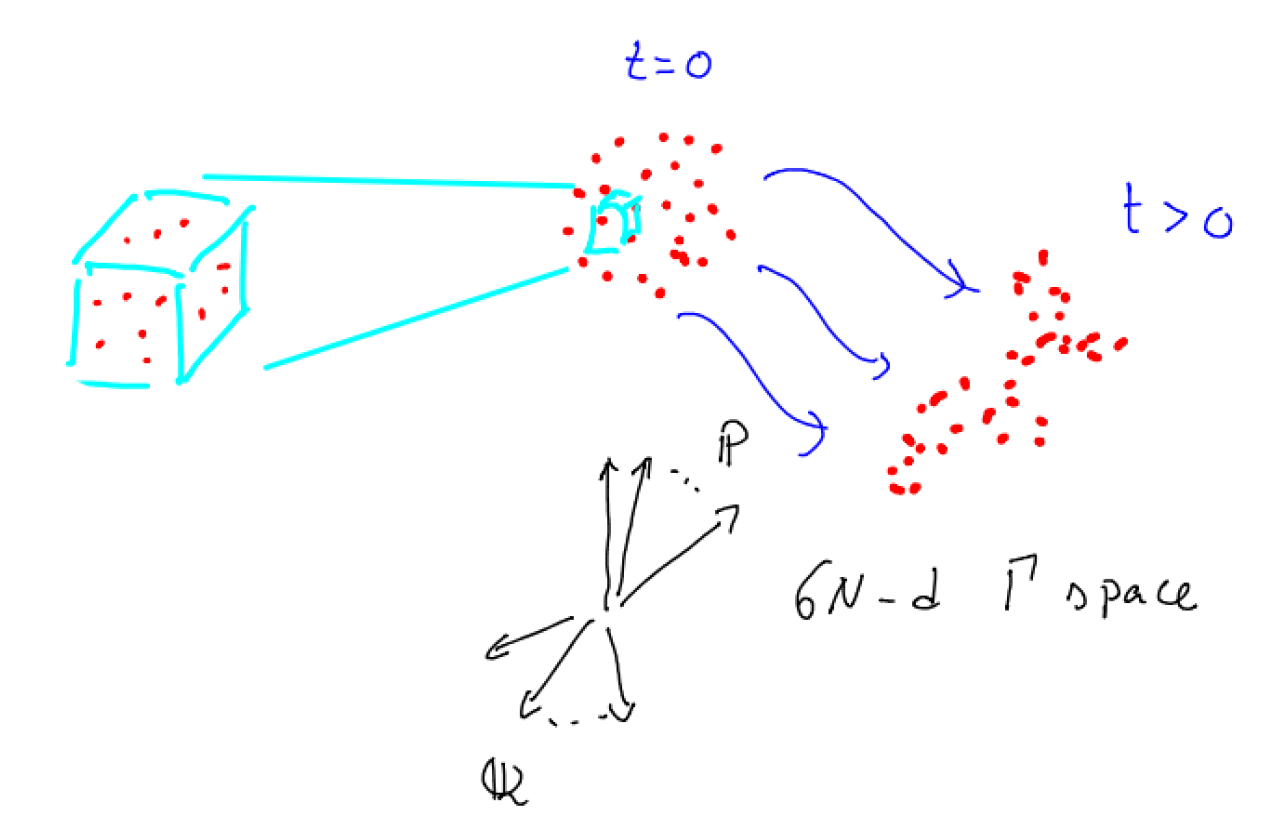
\includegraphics[width=0.7\textwidth]{\main/Images/phase-space-evolution.png}
    \caption{Evolution of an ensemble of system-points in phase space}
    \label{fig:ensemble-evolution}
\end{figure}

By computing how each system-point moves, and then measuring their \textit{density} in phase-space, we can estimate the final probability distribution $\rho(\mathbb{Q},\mathbb{P},t)$, i.e. the \textit{time evolution} of the original ensemble. 

\medskip

Each system-point initially\marginpar{Evolution of a system-point} at $(\mathbb{Q}(0), \mathbb{P}(0))$ \textit{evolves} in time according to the Hamilton equations:
\begin{align}\label{eqn:hamilton-eqs}
    \dot{q}_\alpha &= \pdv{H(\mathbb{Q},\mathbb{P})}{p_\alpha}\qquad \alpha \in \{1x, 1y, 1z,\dots, Nx, Ny, Nz\}\\
    \dot{p}_{\alpha} &= -\pdv{H(\mathbb{Q},\mathbb{P})}{q_\alpha}
\end{align} 
In the simplest case of $N$ point-particles interacting through conservative forces which depend only on their positions, $H$ is given by:
\begin{align*}
    H(\mathbb{Q},\mathbb{P}) = \sum_{i=1}^{3N} \frac{\norm{\bm{p_i}}^2}{2m_i} + U(\mathbb{Q}) 
\end{align*}
In this case (\ref{eqn:hamilton-eqs}) reduces to the second Newton's law:
\begin{align}\label{eqn:newton-eqs}
    m_\alpha \ddot{q}_\alpha = - \pdv{U(\mathbb{Q})}{q_\alpha} \qquad m_\alpha \equiv m_i \text{ if } \alpha \in \{ix,iy,iz\}
\end{align}
A more complicated $H$ can be constructed to describe the motion of more complicated systems, such as \textit{rigid bodies}, or to account more general forces, such as \textit{magnetic ones} (which depend also on $\mathbb{P}$).

\medskip

\textbf{Liouville's theorem}\marginpar{\vspace{4em}Liouville's theorem}\index{Theorem!Liouville} states that the probability density \textit{along a trajectory} does not change during the time evolution: 
\begin{align}\label{eqn:Liouville}
    \dv{t} \rho(\mathbb{Q}(t), \mathbb{P}(t),t) = \pdv{\rho}{t} + \sum_{\alpha=1}^{3N} \left(\pdv{\rho}{q_\alpha} \dot{q}_\alpha + \pdv{\rho}{p_\alpha} \dot{p}_\alpha\right) = 0
\end{align}
where $(\mathbb{Q}(t), \mathbb{P}(t))$ is the solution of (\ref{eqn:hamilton-eqs}) with given initial conditions, and $\dv{t}$ denotes a \textit{total derivative}, taking into account the time-dependence of also $\mathbb{Q}$ and $\mathbb{P}$.  

\medskip

In other words, (\ref{eqn:Liouville}) means that if we follow a system-point during its evolution, and measure the \textit{density} of other system-points travelling in its neighborhood, we will find it unchanging. System-points \textit{do not} \q{coalesce} together, nor \q{disperse} in phase-space --- they behave like droplets of water, flowing and spreading, but never expanding or compressing. In physical terms: probability in phase-space \textit{flows} like an \textit{incompressible fluid}.   

\medskip

Substituting (\ref{eqn:hamilton-eqs}) in (\ref{eqn:Liouville}) and rearranging we get:
\begin{align} \nonumber
    {\pdv{\rho}{t}} (\mathbb{Q}(t), \mathbb{P}(t),t) &= -\sum_{\alpha=1}^{3N} \Bigg[{\pdv{\rho}{q_\alpha}}    (\mathbb{Q}(t), \mathbb{P}(t),t) {\pdv{H}{p_\alpha}}  (\mathbb{Q}(t), \mathbb{P}(t)) + \\   &\quad\>\>\hphantom{\sum_{\alpha=1}^{3N}\Bigg[} - {\pdv{\rho}{p_\alpha}} (\mathbb{Q}(t), \mathbb{P}(t),t) {\pdv{H}{q_\alpha}} (\mathbb{Q}(t), \mathbb{P}(t))
    \Bigg] \label{eqn:liouville-hamilton} 
\end{align}

Note that in (\ref{eqn:Liouville}) we can fix any point $(\mathbb{Q},\mathbb{P})$ and then find some appropriate initial conditions $(\mathbb{Q}(0), \mathbb{P}(0))$ such that the trajectory will pass through that point at time $t$, i.e. $(\mathbb{Q}(t), \mathbb{P}(t)) = (\mathbb{Q},\mathbb{P})$. 

In this way we can remove\marginpar{\vspace{4em}Liouville operator for time evolution} the time-dependence of $\mathbb{Q}(t)$ and $\mathbb{P}(t)$ in (\ref{eqn:liouville-hamilton}), leading to:
\begin{align}\label{eqn:liouville-hamilton-no-dep}
    \pdv{t} \rho(\mathbb{Q},\mathbb{P},t) &= - \sum_{\alpha=1}^{3N} \left[{\pdv{\rho}{q_\alpha}}
     (\mathbb{Q},\mathbb{P},t) {\pdv{H}{p_\alpha}}  (\mathbb{Q},\mathbb{P})
    - {\pdv{\rho}{p_\alpha}} (\mathbb{Q},\mathbb{P},t) {\pdv{H}{q_\alpha}} (\mathbb{Q},\mathbb{P})
    \right] =\\ \nonumber
    &\equiv - \{\rho, H\} = -i \hat{L} \rho
\end{align}
Where $\{\cdot, \cdot\}$ is the so-called \textbf{Poisson bracket}:
\begin{align*}
    \{f,g\} \equiv \sum_{i=1}^n \left(\pdv{f}{q_i} \pdv{g}{p_i} - \pdv{f}{p_i} \pdv{g}{q_i}\right)
\end{align*} 
and $\hat{L}$ is a linear operator called as the \textit{Liouvillian} (or \textbf{Liouville operator}\index{Operator!Liouvillian}):
\begin{align*}
    i \hat{L} \equiv \{\cdot, H\}
\end{align*}

We can then use (\ref{eqn:liouville-hamilton-no-dep}) as an evolution equation to compute $\rho(\mathbb{Q},\mathbb{P},t)$ given an initial condition $\rho(\mathbb{Q},\mathbb{P},0) \equiv \rho_0(\mathbb{Q},\mathbb{P})$ for any $t > 0$.

Since it is a linear differential equation in time, its formal solution can be written in terms of the \textit{exponential} of the operator $\hat{L}$:
\begin{align*}
    \rho(\mathbb{Q},\mathbb{P},t) = e^{-i \hat{L} t} \rho_0(\mathbb{Q},\mathbb{P})
\end{align*} 

\begin{proof}
    \marginpar{\textbf{Proof} of Liouville's theorem}
    The idea is to compute explicitly the derivative in (\ref{eqn:liouville-hamilton-no-dep}).
    
    \medskip
    
    The probability density $\rho(\mathbb{Q},\mathbb{P},t)$ at a given instant $t$ can be obtained by \textit{counting} all system-points that arrive at $(\mathbb{Q},\mathbb{P})$ \textit{from every possible origin} $(\mathbb{Q}_0,\mathbb{P}_0)$, weighting each of them with its \q{origin probability} $\rho_0(\mathbb{Q}_0, \mathbb{P}_0)$:
    \begin{align}\label{eqn:9}
        \rho(\mathbb{Q},\mathbb{P},t) = \int_{\bm{\Gamma}} \underbrace{\dd[3N]{\bm{q_0}} \dd[3N]{\bm{p_0}} }_{\dd{\Gamma_0} } \delta^{3N} (\mathbb{Q}(t)- \mathbb{Q}) \> \delta^{3N}(\mathbb{P}(t) - \mathbb{P}) \> \rho_0(\mathbb{Q}_0, \mathbb{P}_0)
    \end{align}
    In this notation, $\delta^{3N}$ is the \textit{product} of $3N$ $\delta$\textit{s}. For example, for the positions we have:  %Not very rigorous, it should be just a single delta
    \begin{align*}
        \delta^{3N}(\mathbb{Q}(t) - \mathbb{Q}) \equiv \prod_{\alpha=1}^{3N} \delta(q_\alpha(t) - q_\alpha) 
    \end{align*}
    and a similar expression holds for the momenta.

    On the other hand, $\mathbb{Q}_0$, $\mathbb{P}_0$ are the initial conditions for the motion $(\mathbb{Q}(t), \mathbb{P}(t))$, i.e. $(\mathbb{Q}(t=0), \mathbb{P}(t=0)) = (\mathbb{Q}_0, \mathbb{P}_0)$. So, in the integral (\ref{eqn:9}) the $(\mathbb{Q}(t), \mathbb{P}(t))$ \textbf{depend} (implicitly) on the origin coordinates $(\mathbb{Q}_0, \mathbb{P}_0)$. 

    In the following, to simplify notation, we denote $\dd{\Gamma_0} \equiv \dd[3N]{\bm{q_0}} \dd[N]{\bm{p_0}}$. 

    \medskip

    Differentiating (\ref{eqn:9}) with respect to $t$ we get:
    \begin{align}\nonumber
        \pdv{t} \rho(\mathbb{Q},\mathbb{P},t) &= \pdv{t} \int_{\bm{\Gamma}} \dd{\Gamma_0} \delta^{3N}(\mathbb{Q}(t)-\mathbb{Q}) \> \delta^{3N}(\mathbb{P}(t)-\mathbb{P}) \> \rho_0(\mathbb{Q}_0,\mathbb{P}_0) =\\ \nonumber
        &\underset{(a)}{=}  \textcolor{Red}{-} \int_{\bm{\Gamma}} \dd{\Gamma_0} \rho_0(\mathbb{Q}_0, \mathbb{P}_0) \sum_{\alpha=1}^{3N} \left[\dot{q}_\alpha(t) \pdv{q_\alpha} + \dot{p}_\alpha(t) \pdv{p_\alpha}\right] \cdot  \\
        &\quad\> \cdot \delta^{3N}(\mathbb{Q}(t) - \mathbb{Q}) \> \delta^{3N}(\mathbb{P}(t) - \mathbb{P}) \label{eqn:10}
    \end{align}
    The $-$ sign comes from the definition of \textit{distributional derivative} - see the following green box for more information. 

    \begin{expl}\textbf{Derivative of the Dirac-delta}. 
    $\delta$ is a \textit{distribution}, and so its derivative is defined by its \textit{action} on test functions $\varphi \in \mathcal{S}(\mathbb{R})$:
    \begin{align*}
        \langle \delta', \varphi \rangle \equiv - \langle \delta, \varphi' \rangle = -\varphi'(0) \qquad \forall \varphi \in \mathcal{S}(\mathbb{R})
    \end{align*}  
    This definition is motivated by the following \textit{formal} manipulation:
    \begin{align*}
        \langle \delta', \varphi \rangle = \int_{\mathbb{R}} \dd{x} \delta'(x) \varphi(x) \quad\underset{\mathclap{\rm{by\ parts}}}{=}\quad \cancel{ \varphi(x) \delta(x) }\Big|_{x=-\infty}^{x=+\infty} - \int_{\mathbb{R}} \dd{x} \delta(x)  \varphi'(x) = -\varphi'(0)
    \end{align*} 

    The same relation can be generalized to partial derivatives in higher dimension. For example, let $\bm{r} = (x, y, z)^T$. Then:
    \begin{align*}
        \langle \pdv{x} \delta^3, \varphi \rangle \equiv - \pdv{x} \varphi( \bm{0}) \qquad \forall \varphi \in \mathcal{S}(\mathbb{R}^3)
    \end{align*}
    If the argument of the delta is shifted, so it will be in the result. Let $\delta^3_{\bm{r_0}} \equiv \delta(\bm{r} - \bm{r_0})$. Then:
    \begin{align} \label{eqn:delta-shift}
        \langle \pdv{x} \delta^3_{\bm{r_0}}, \varphi \rangle \equiv -\pdv{x} \varphi(\bm{r_0})
    \end{align}
    Let's consider the time-derivative of just one of the $\delta$\textit{s} in (\ref{eqn:10}):
    \begin{align*}
        \pdv{t} \delta(q_\alpha(t) - q_\alpha)
    \end{align*} 
    To compute it, we apply it to a test function $\varphi(x) \in \mathcal{S}(\mathbb{R})$, and apply definition (\ref{eqn:delta-shift}):
    \begin{align}\nonumber
        \langle \pdv{t} \delta(q_\alpha(t)-q_\alpha), \varphi \rangle &= -\pdv{t} \varphi(q_\alpha(t)) = -\left(\pdv{q_\alpha} \varphi(q_{\alpha}(t))\right) \dot{q}_\alpha(t) =\\ \label{eqn:delta-res}
        &\equiv -\langle \dot{q}_\alpha(t) \pdv{q_\alpha} \delta(q_\alpha(t)-q_\alpha), \varphi\rangle
    \end{align}
    And so we get the following identity between operators:
    \begin{align*}
        \pdv{t}\delta(q_{\alpha}(t) - q_\alpha) = - \dot{q}_\alpha(t) \pdv{q_\alpha} \delta(q_{\alpha}(t) - q_\alpha)
    \end{align*}
    Another way to see (\ref{eqn:delta-res}) is by \textit{formally} writing:
    \begin{align*}
        \langle \pdv{t} \delta(q_{\alpha}(t) - q_\alpha), \varphi \rangle &= \int_{\mathbb{R}} \dd{q_\alpha} \pdv{t} \delta(q_{\alpha}(t)-q_\alpha) \varphi(q_{\alpha})
        \shortintertext{Here the $\partial_t$ acts on \textit{everything} on its right, i.e. $\partial_t \delta(\cdots) \varphi$ is to be intended as first applying $\delta$ to the $\varphi$, and then $\partial_t$ to the result. As $\partial_t$ acts on the entire integral, we can bring it out:}
        &= \pdv{t} \int_{\mathbb{R}} \dd{q_\alpha} \delta(q_{\alpha}(t) - q_\alpha) \varphi(q_\alpha) =\\
        &= \pdv{t} \varphi(q_\alpha(t)) = (\ref{eqn:delta-res})
    \end{align*} 

    To extend to more dimensions (e.g. $3$), we need to use gradients when applying the chain rule. For example, for $d=3$ and $\mathbb{R}^3 \ni \bm{r} \mapsto \varphi(\bm{r})$:
    \begin{align*}
        \langle \pdv{t} \delta^3(\bm{r}(t) - \bm{r}), \varphi\rangle &= -\pdv{t} \varphi(\bm{r}(t)) = -\grad_{\bm{r}} \varphi(\bm{r}(t)) \cdot \dot{\bm{r}}(t) =\\
        &= - \sum_{i=1}^3 \dot{r}_i(t) \pdv{r_i} \varphi(\bm{r}(t))
    \end{align*}
    In operator terms:
    \begin{align*}
        \pdv{t}\delta^3(\bm{r}(t)-\bm{r}) = -\dot{\bm{r}}(t) \cdot \grad_{\bm{r}} \delta(\bm{r}(t) - \bm{r})
    \end{align*}

    In step (a) of (\ref{eqn:10}) we are dealing with $6N$ coordinates at once:
    \begin{align*}
        \pdv{t} \delta^{6N}[(\mathbb{Q}(t), \mathbb{P}(t)) - (\mathbb{Q},\mathbb{P})] &= -(\dot{\mathbb{Q}}(t), \dot{\mathbb{P}}(t)) \cdot \grad_{(\bm{\mathbb{Q}}, \bm{\mathbb{P}})} \delta^{6N}[(\mathbb{Q}(t), \mathbb{P}(t)) - (\mathbb{Q},\mathbb{P})] =\\
        =\textcolor{Red}{-} \left\{\sum_{\alpha=1}^{3N} \left[\dot{q}_\alpha(t) \pdv{q_\alpha} + \dot{p}_\alpha(t) \pdv{p_\alpha}\right] \right\} \delta^{3N}(\mathbb{Q}(t) - \mathbb{Q}) \>  \delta^{3N}(\mathbb{P}(t) - \mathbb{P}) \span
    \end{align*}
    where $(\mathbb{Q}(t), \mathbb{P}(t))$ denotes the $6N$-dimensional vector with the first $3N$ entries equal to the ones of $\mathbb{Q}(t)$, and the last ones equal to those of $\mathbb{P}(t)$.
        
    \end{expl}

    In (\ref{eqn:10}) we then use (\ref{eqn:hamilton-eqs}) to rewrite the $\dot{q}_\alpha(t)$ and $\dot{p}_\alpha(t)$:
    \begin{align} \nonumber
        \pdv{t} \rho(\mathbb{Q},\mathbb{P},t) &= - \int_{\bm{\Gamma}} \dd{\Gamma_0} \rho_0(\mathbb{Q}_0, \mathbb{P}_0) \sum_{\alpha=1}^{3N} \Bigg[{\pdv{H}{p_\alpha}} (\mathbb{Q}(t), \mathbb{P}(t)) \pdv{q_\alpha} + \\ \nonumber
        &\quad \> - {\pdv{H}{q_\alpha}} (\mathbb{Q}(t), \mathbb{P}(t)) \pdv{p_\alpha}\Bigg] \delta^{3N}(\mathbb{Q}(t) - \mathbb{Q}) \> \delta^{3N}(\mathbb{P}(t) - \mathbb{P}) =
        \shortintertext{The two $\delta$\textit{s} \textit{fix} the arguments of $H$ and its derivatives to $(\mathbb{Q},\mathbb{P})$:} \nonumber
        &= -\int_{\bm{\Gamma}} \dd{\Gamma_0} \rho_0(\mathbb{Q}_0, \mathbb{P}_0) \textcolor{Blue}{\sum_{\alpha=1}^{3N} \left[{\pdv{H}{p_\alpha}} (\mathbb{Q},\mathbb{P}) \pdv{q_\alpha} - {\pdv{H}{q_\alpha}} (\mathbb{Q},\mathbb{P}) \pdv{p_\alpha}\right]} \cdot\\ \nonumber
        &\qquad\quad \cdot \delta^{3N}(\mathbb{Q}(t) - \mathbb{Q}) \> \delta^{3N} (\mathbb{P}(t) - \mathbb{P}) =
        \shortintertext{Now the sum (highlighted in blue) is independent of the integration variable, and so can be brought outside of the integral:} \nonumber
        &= -\sum_{\alpha=1}^{3N} \left[{\pdv{H}{p_\alpha}} (\mathbb{Q}, \mathbb{P}) \pdv{q_\alpha} - {\pdv{H}{q_\alpha}} (\mathbb{Q},\mathbb{P}) \pdv{p_\alpha}\right] \cdot \\ 
        &\qquad \> \cdot \underbrace{\int_{\bm{\Gamma}} \dd{\Gamma_0} \rho_0(\mathbb{Q}_0, \mathbb{P}_0) \> \delta^{3N}(\mathbb{Q}(t) - \mathbb{Q}) \> \delta^{3N} (\mathbb{P}(t) - \mathbb{P})}_{\rho(\mathbb{Q},\mathbb{P},t) \quad (\ref{eqn:9})} \label{eqn:9-bis}
    \end{align}
    This last result (\ref{eqn:9-bis}) can be rewritten as:
    \begin{align*}
        \pdv{t} \rho(\mathbb{Q},\mathbb{P},t) = - \{\rho(\mathbb{Q},\mathbb{P},t), H(\mathbb{Q}, \mathbb{P})\}
    \end{align*}
    which is exactly eq. (\ref{eqn:liouville-hamilton-no-dep}). Substituting into the total derivative completes the proof:
    \begin{align*}
        \dv{t} \rho(\mathbb{Q}(t), \mathbb{P}(t), t) \underset{\mathclap{(\ref{eqn:Liouville})}}{=} \pdv{\rho}{t} + \{\rho,H\} = -\{\rho,H\} + \{\rho,H\} = 0
    \end{align*}
\end{proof}

\begin{exo}[Liouville's theorem]
    Show that (\ref{eqn:liouville-hamilton-no-dep}) implies (\ref{eqn:Liouville}).

    \medskip

    \textbf{Solution}. We start by computing the total derivative of $\rho(\mathbb{Q}(t), \mathbb{P}(t),t)$ with respect to time $t$:
    \begin{align*}
        \dv{t} \rho(\mathbb{Q}(t), \mathbb{P}(t),t) &= \sum_{\alpha=1}^{3N} \left[ {\pdv{\rho}{q_\alpha}} (\mathbb{Q}(t), \mathbb{P}(t),t) \dot{q}_\alpha(t) + {\pdv{\rho}{p_\alpha}} (\mathbb{Q}(t), \mathbb{P}(t),t) \dot{p}_\alpha(t)\right] +\\
        &\quad \> +  {\pdv{\rho}{t}} (\mathbb{Q}(t), \mathbb{P}(t),t)
        \shortintertext{We rewrite $\dot{q}_\alpha$ and $\dot{p}_\alpha$ through the Hamilton equations (\ref{eqn:hamilton-eqs}):}
        &= \sum_{\alpha=1}^{3N} \Bigg[{\pdv{\rho}{q_\alpha}} (\mathbb{Q}(t), \mathbb{P}(t),t) {\pdv{H}{p_\alpha}} (\mathbb{Q}(t),\mathbb{P}(t)) + \\
        &\qquad \qquad -{\pdv{\rho}{p_\alpha}} (\mathbb{Q}(t), \mathbb{P}(t), t) {\pdv{H}{q_\alpha}} (\mathbb{Q}(t), \mathbb{P}(t))  \Bigg] + \\
        &\qquad \> +{\pdv{\rho}{t}} (\mathbb{Q}(t), \mathbb{P}(t), t)
    \end{align*}
    Using (\ref{eqn:liouville-hamilton-no-dep}) for the last term we have:
    \begin{align*}
        {\pdv{\rho}{t}} (\mathbb{Q}(t), \mathbb{P}(t), t) &= - \sum_{\alpha=1}^{3N} \Bigg[ {\pdv{\rho}{q_\alpha}} (\mathbb{Q}(t), \mathbb{P}(t), t) {\pdv{H}{p_\alpha}} (\mathbb{Q}(t), \mathbb{P}(t)) +\\
        &\qquad \qquad - {\pdv{\rho}{p_\alpha}} (\mathbb{Q}(t), \mathbb{P}(t),t) {\pdv{H}{q_\alpha}} (\mathbb{Q}(t), \mathbb{P}(t))  \Bigg]
    \end{align*}
    which leads to a total cancellation, and so:
    \begin{align*}
        \dv{t} \rho(\mathbb{Q}(t), \mathbb{P}(t), t) \equiv 0 \qquad \forall t
    \end{align*}
    as desired.
\end{exo}

\subsection{Measure theoretic version}
We can express the results of Liouville's theorem in terms of the (hyper)\textit{volumes} occupied by system-points in phase-space \cite[Appendix~A]{mathsm}. As we have noted before, an ensemble \textit{evolves} like an \textit{incompressible fluid}. So, as a cup of water \textit{does not change its total volume} after being stirred or scattered or dispersed, so do the ensembles experiencing Hamiltonian evolution.

\medskip

Let's make this more precise. Consider a Lebesgue-measurable subset $A_0 \subset \Gamma$ of phase-space. Then we have a way to compute its \textit{measure} (a generalization of \q{volume}) with the integral:
\begin{align*}
    V(A_0) \equiv \int_{A_0} \dd[3N]{\bm{q}} \dd[3N]{\bm{p}} \equiv \int_{A_0} \dd{\Gamma_0}
\end{align*} 
Let $A_0$ evolve for a time $t$ \marginpar{Measure-theoretic \textbf{Liouville's theorem}}according to Hamilton equations (\ref{eqn:hamilton-eqs}), and call its \textit{evolved} version $A_t$. Then we can restate \textbf{Liouville's theorem} as the equality:
\begin{align}\label{eqn:Liouville-volumes}
    V(A_0) = V(A_t) \qquad \forall t
\end{align} 

Before providing a formal proof,\marginpar{Heuristic proof} consider the following \textit{heuristic} considerations. Let $A$ be a sufficiently small region of phase-space (obtained, for example, by partitioning a larger region $B$), so that the density of system-points in it is (approximately) constant: $\rho(\mathbb{Q},\mathbb{P},t) \approx \mathrm{const} \neq 0$. Let $A_t$ be its \textit{evolved} version after time $t$. The fraction $\Delta N_t$ of system-points inside $A_t$ is given by:
\begin{align*}
    \Delta N_t = \rho(\mathbb{Q}(t), \mathbb{P}(t), t) V(A_t)
\end{align*}
and remains constant by definition. Differentiating with respect to $t$:
\begin{align*}
    0 \equiv \dv{t} \Delta N_t = \underbrace{\dv{\rho}{t} (\mathbb{Q}(t), \mathbb{P}(t), t) \cdot V(A_t)}_{\mathclap{0 \text{ by Liouville's theorem}}} + \rho(\mathbb{Q}(t), \mathbb{P}(t), t) \dv{t} V(A_t)
\end{align*}
Dividing by $\rho$ we obtain:
\begin{align*}
    \dv{V}{t} (A_t) = 0
\end{align*}
Meaning that the volume of $A_t$ does not change, and so:
\begin{align*}
    V(A_t) = V(A_0)
\end{align*}

\medskip

%Liouville theorem can be used to explain irreversibility and the emergence of time
\begin{proof}
    Let's \textit{formalize} this argument. We focus on proving that the Liouville's theorem (\ref{eqn:Liouville}) implies (\ref{eqn:Liouville-volumes}). \marginpar{Formal proof}.  
    
    \medskip

    We start by writing $V(A_0)$ as an integral. First, we express the two regions $A_0$ and $A_t$ as uniform densities:
    \begin{align*}
        \rho_0(\mathbb{Q}, \mathbb{P}) = \bb{1}_{A_0} (\mathbb{Q}, \mathbb{P}); \qquad \rho(\mathbb{Q},\mathbb{P},t) = \bb{1}_{A_t} (\mathbb{Q},\mathbb{P})
    \end{align*}
    Then, the volume of $A_0$ is given by:
    \begin{align} \nonumber
        V(A_0) &= \int_{\bm{\Gamma}} \dd[3N]{\bm{q}} \dd[3N]{\bm{p}} \rho_0(\mathbb{Q}, \mathbb{P}) =
    \shortintertext{And we rename the integration variables to $\bm{q_0}$ and $\bm{p_0}$:}
    &= \int_{\bm{\Gamma}} \dd[3N]{\bm{q_0}} \dd[3N]{\bm{p_0}} \rho_0(\mathbb{Q}_0, \mathbb{P}_0) \label{eqn:pk1}
    \intertext{By Liouville's theorem (\ref{eqn:Liouville}), the local density does not change along a path. In particular, consider the path starting at $(\mathbb{Q}_0, \mathbb{P}_0)$ and arriving at $(\mathbb{Q}(t; \mathbb{Q}_0, \mathbb{P}_0), \mathbb{P}(t; \mathbb{Q}_0, \mathbb{P}_0))$ at time $t$, i.e. such that:} \nonumber
    \mathbb{Q}(t; \mathbb{Q}_0, \mathbb{P}_0) \Big|_{t=0} = \mathbb{Q}_0; \qquad \mathbb{P}(t; \mathbb{Q}_0, \mathbb{P}_0) \Big|_{t=0} = \mathbb{P}_0 \span
    \shortintertext{Since density does not change along a path:} \nonumber
        \rho(\mathbb{Q}(t; \mathbb{Q}_0, \mathbb{P}_0), \mathbb{P}(t; \mathbb{Q}_0, \mathbb{P}_0), t) = \rho_0(\mathbb{Q}_0, \mathbb{P}_0) \span
    \end{align}
    Substituting in (\ref{eqn:pk1}) leads to:
    \begin{align*}
        V(A_0) = \int_{\bm{\Gamma}} \dd[3N]{\bm{q_0}} \dd[3N]{\bm{\rho_0}} \> \rho(\mathbb{Q}(t;\mathbb{Q}_0, \mathbb{P}_0), \mathbb{P}(t; \mathbb{Q}_0, \mathbb{P}_0), t)
    \end{align*}
    Then we change variables, passing from the origin $(\mathbb{Q}_0, \mathbb{P}_0)$ to an arbitrary end-point $(\mathbb{Q},\mathbb{P})$:
    \begin{align}\label{eqn:kp2}
        (\mathbb{Q}, \mathbb{P}) = (\mathbb{Q}(t; \mathbb{Q}_0, \mathbb{P}_0), \mathbb{P}(t; \mathbb{Q}_0, \mathbb{P}_0))
    \end{align}
    leading to:
    \begin{align*}
        V(A_0) = \int_{\bm{\Gamma}} \dd[3N]{\bm{q}} \dd[3N]{\bm{p}} \rho(\mathbb{Q}, \mathbb{P}, t) J^{-1} 
    \end{align*}
    where the determinant $J$ of the Jacobian of the change of variables is given by:
    \begin{align*}
        J = \operatorname{det}\left| \pdv{(\mathbb{Q}, \mathbb{P})}{(\mathbb{Q}_0, \mathbb{P}_0)}\right|
    \end{align*}
    If $J = 1$, then (\ref{eqn:kp2}) would become:
    \begin{align*}
        V(A_0) = \int_{\bm{\Gamma}} \dd[3N]{\bm{q}} \dd[3N]{\bm{p}} \underbrace{\rho(\mathbb{Q}, \mathbb{P}, t)}_{\bb{1}_{A_t}(\mathbb{Q}, \mathbb{P})} = V(A_t)
    \end{align*} 
    thus concluding the theorem.

    \medskip

    So, all that's left is to verify that the following determinant is unitary:
    \begin{align*}
        J(t) = \operatorname{det}\left| \pdv{(\mathbb{Q}(t; \mathbb{Q}_0, \mathbb{P}_0), \mathbb{P}(t; \mathbb{Q}_0, \mathbb{P}_0))}{(\mathbb{Q}_0, \mathbb{P}_0)}\right|
    \end{align*}
    where $\mathbb{Q}(t)$ and $\mathbb{P}(t)$ are obtained with the Hamilton equations (\ref{eqn:hamilton-eqs}). 

    \medskip

    For simplicity of notation, let's define:
    \begin{align}\label{eqn:simplicity-not}
        (\mathbb{Q}_0, \mathbb{P}_0) \equiv \bm{y}; \qquad (\mathbb{Q}(t; \mathbb{Q}_0, \mathbb{P}_0), \mathbb{P}(t; \mathbb{Q}_0, \mathbb{P}_0)) \equiv \bm{x}(t, \bm{y})
    \end{align}
    And so:
    \begin{align*}
        J(t) = \operatorname{det}\left| \pdv{(x_1,\dots, x_{6N})}{(y_1, \dots, y_{6N})}\right|
    \end{align*}
    We already know that $J(0) = 1$, because $\bm{x}(0,\bm{y}) = \bm{y}$. So, if we prove that $J(t)$ is constant, i.e. it does not depend on $t$, we will have $J(t) \equiv 1$, as desired. The idea is thus to \textit{differentiate} $J(t)$ and use Hamilton equations (\ref{eqn:hamilton-eqs}).
    
    \medskip

    In general, for a matrix $A(t)$ with rows $(\bm{A_{1}}(t), \dots, \bm{A_{n}}(t))^T$, we have:    
    \begin{align} \nonumber
        \dv{t}\operatorname{det} A(t) &= \dv{t} \operatorname{det} \scalebox{0.8}{$\begin{vmatrix}
            \text{|---} & \bm{A_1}(t) & \text{---|} \\
            \text{|---} & \bm{A_2}(t) & \text{---|} \\
            & \vdots & \\
            \text{|---} & \bm{A_n}(t) & \text{---|} 
        \end{vmatrix}$} = \\ \nonumber
        &= \operatorname{det} \scalebox{0.8}{$\begin{vmatrix}
            \text{|---} & \textcolor{Red}{\bm{A_1}'(t)} & \text{---|} \\
            \text{|---} & \bm{A_2}(t) & \text{---|} \\
            & \vdots & \\
            \text{|---} & \bm{A_n}(t) & \text{---|} 
        \end{vmatrix}$} + \operatorname{det} \scalebox{0.8}{$\begin{vmatrix}
            \text{|---} & \bm{A_1}(t) & \text{---|} \\
            \text{|---} & \textcolor{Red}{\bm{A_2}'(t)} & \text{---|} \\
            & \vdots & \\
            \text{|---} & \bm{A_n}(t) & \text{---|} 
        \end{vmatrix}$} + \dots + \operatorname{det} \scalebox{0.8}{$\begin{vmatrix}
            \text{|---} & \bm{A_1}(t) & \text{---|} \\
            & \vdots & \\
            \text{|---} & \bm{A_{n-1}}(t) & \text{---|} \\
            \text{|---} & \textcolor{Red}{\bm{A_n}'(t)} & \text{---|} 
        \end{vmatrix}$} = \\
        &= \sum_{i=1}^n \operatorname{det}[(\bm{A_1}(t), \dots, \bm{A_{i-1}}(t), \bm{A_i}'(t), \bm{A_{i+1}}(t), \dots, \bm{A_n}(t) )^T] \label{eqn:det-dot}
    \end{align}
    For a proof of (\ref{eqn:det-dot}) see the green box at pag. \pageref{proof:det-dot}.
    
    In our case, (\ref{eqn:det-dot}) leads to:
    \begin{align}\label{eqn:dvJ}
        \dv{t} J(t) = \sum_{i=1}^{6N} \operatorname{det}\left|\pdv{(x_1, \dots, x_{i-1}, \dot{x}_i, x_{i+1}, \dots, x_{6N})}{(y_1, \dots, y_{i-1}, y_i, y_{i+1}, \dots, y_{6N})}\right| \equiv \sum_{i=1}^{6N} \operatorname{det} A_i 
    \end{align} 
    where $x_i = q_i$ for $1 \leq i \leq 3N$, and $p_i$ for $3N < i \leq 6N$. In either case, when we differentiate and compute $\dot{x}_i$, we will have, as consequence of (\ref{eqn:hamilton-eqs}) one of the two results:
    \begin{align*}
        \dot{q}_\alpha = \pdv{H}{p_\alpha}; \qquad \dot{p}_\alpha = - \pdv{H}{q_\alpha}
    \end{align*}
    which are both functions of $(\mathbb{Q}, \mathbb{P})$, i.e. of $\bm{x}$. Thus, the $(i,k)$ elements of such matrices can be computed by the chain-rule:
    \begin{align}
        \pdv{\dot{x}_i}{y_k} = \sum_{j=1}^{6N} \pdv{\dot{x}_i}{x_j} \pdv{x_j}{y_k} 
    \end{align}
    In vector notation:
    \begin{align} \label{eqn:xidot}
        \pdv{\dot{x}_i}{\bm{y}} = \sum_{j=1}^{6N} \pdv{\dot{x_i}}{x_j} \pdv{x_j}{\bm{y}}
    \end{align}
    Note that $\pdv{\dot{x}_i}{\bm{y}}$ is the $i$-th row of the matrix $A_i$, which, according to (\ref{eqn:xidot}), can be written as a sum of $6N$ rows. As all other rows of $A_i$ remain unchanged, we can use the \textit{row-linearity} of the determinant (see (\ref{eqn:prop1}) and (\ref{eqn:prop2})):
    \begin{align*}
        \operatorname{det} A_i &= \operatorname{det} \scalebox{0.9}{$\begin{vmatrix}
            \text{|---} & \pdv{x_1}{\bm{y}} & \text{---|} \\
            & \vdots & \\
            \text{|---} & \pdv{x_{i-1}}{\bm{y}} & \text{---|}\\
            \text{|---} & \displaystyle \sum_{i=1}^{6N} \pdv{\dot{x_i}}{x_j} \pdv{x_j}{\bm{y}} & \text{---|}\\
            \text{|---} & \pdv{x_{i+1}}{\bm{y}} & \text{---|}\\
            & \vdots & \\
            \text{|---} & \pdv{x_{6N}}{\bm{y}} & \text{---|} 
        \end{vmatrix}$} = \sum_{j=1}^{6N} \pdv{\dot{x_i}}{x_j} \operatorname{det} \scalebox{0.9}{$\begin{vmatrix}
            \text{|---} & \pdv{x_1}{\bm{y}} & \text{---|} \\
            & \vdots & \\
            \text{|---} & \pdv{x_{i-1}}{\bm{y}} & \text{---|}\\
            \text{|---} &\displaystyle  \pdv{x_j}{\bm{y}} & \text{|---}\\
            \text{|---} & \pdv{x_{i+1}}{\bm{y}} & \text{---|}\\
            & \vdots & \\
            \text{|---} & \pdv{x_{6N}}{\bm{y}} & \text{---|} 
        \end{vmatrix}$} =\\
        &= \sum_{j=1}^{6N} \pdv{\dot{x}_i}{x_j} \underbrace{\operatorname{det}\left| \pdv{(x_1, \dots, x_{i-1}, \textcolor{Red}{x_j}, x_{i+1}, \dots, x_{6N})}{(y_1, \dots, y_{i-1}, y_i, y_{i+1}, \dots, y_{6N})}\right|}_{\delta_{ij} J} 
        \intertext{The determinant in the sum argument is obtained by replacing the $i$-th row of the jacobian in $J$ with the $j$-th. But if there are two repeated rows, the determinant will be $0$. So the only non-zero possibility is when $j=i$, and in that case the determinant will be exactly $J$. This leads to a Kronecker delta $\delta_{ij}$ that we can use to collapse the sum, leading to:}
        \operatorname{det} A_i &= \pdv{\dot{x}_i}{x_i} J 
    \end{align*}
    Substituting this last result back in (\ref{eqn:dvJ}) we get:
    \begin{align*}
        \dv{J}{t} = J \sum_{i=1}^{6N} \pdv{\dot{x}_i}{x_i}
    \end{align*}

    We then undo the change of variables (\ref{eqn:simplicity-not}), splitting the first and last $3N$ terms of the sum:
    \begin{align*}
        \sum_{i=1}^{6N} \pdv{\dot{x}_i}{x_i} = \sum_{\alpha=1}^{3N} \left[\pdv{q_\alpha} \dot{q}_\alpha + \pdv{p_\alpha} \dot{p}_\alpha\right] \underset{(\ref{eqn:hamilton-eqs})}{=} \sum_{\alpha=1}^{3N} \left[\pdv{q_\alpha} \pdv{H}{p_\alpha} + \pdv{p_\alpha} \left(-\pdv{H}{q_\alpha}\right)\right] = 0
    \end{align*}
    And so:
    \begin{align*}
        \dv{J}{t} \equiv 0
    \end{align*}
    meaning that $J(t)$ is constant, and then, as noted before:
    \begin{align*}
        J(t) = J(0) = 1
    \end{align*}
    which proves Liouville's theorem.

\end{proof}

\begin{expl}\textbf{Derivative of a determinant} \textit{(Proof of}(\ref{eqn:det-dot})\textit{)}.\label{proof:det-dot} 

    We start by noting that the determinant of a matrix $A$ is a linear function of its rows or columns. For example, if $A \in \mathcal{M}(\mathbb{R}^{d \times d})$ has rows $\{\bm{A_i}\}_{i=1,\dots,n}$, then the following two relations hold:
    \begin{align} \label{eqn:prop1}
        \operatorname{det}|(\bm{A_1},\dots,\bm{A_{i-1}}, \textcolor{Red}{\lambda}\bm{A_i}, \bm{A_{i+1}}\dots, \bm{A_n})^T| = \\ \nonumber
       \textcolor{Red}{\lambda} \operatorname{det} | (\bm{A_1},\dots,\bm{A_{i-1}}, \bm{A_i} , \bm{A_{i+1}}\dots, \bm{A_n})^T| \qquad \forall 1 \leq i \leq n; \> \forall \lambda \in \mathbb{R} \span
    \end{align}
    \begin{align} \label{eqn:prop2}
       &\operatorname{det}|(\bm{A_1},\dots,\bm{A_{i-1}}, \bm{A_i} + \textcolor{Red}{\bm{w}}, \bm{A_{i+1}}\dots, \bm{A_n})^T| = \\ \nonumber
       &\hphantom{+}\operatorname{det} | (\bm{A_1},\dots,\bm{A_{i-1}}, \bm{A_i} , \bm{A_{i+1}}\dots, \bm{A_n})^T| +\\ \nonumber
       &\operatorname{+det} | (\bm{A_1},\dots,\bm{A_{i-1}}, \textcolor{Red}{\bm{w}}, \bm{A_{i+1}}\dots, \bm{A_n})^T|
       \qquad \forall 1 \leq i \leq n; \> \forall \bm{w} \in \mathbb{R}^d 
    \end{align}
    This property is proved geometrically in fig. \ref{fig:det-linear}.

    \medskip

    We then proceed by computing the time derivative of $\operatorname{det} A(t)$ as the limit of the difference quotient:
    \begin{align} \nonumber
        \dv{t} \operatorname{det}A(t) &\equiv \lim_{\Delta t \to 0} \frac{\operatorname{det} A(t+\Delta t) - \operatorname{det} A(t)}{\Delta t} = 
    \shortintertext{In terms of rows:} \nonumber
        &= \lim_{\Delta t \to 0} \frac{1}{\Delta t} \Bigg( \operatorname{det} \scalebox{0.8}{$\begin{vmatrix}
            \text{|---} & \bm{A_1}(t + \Delta t) & \text{---|} \\
            & \vdots & \\
            \text{|---} & \bm{A_n}(t + \Delta t) & \text{---|} 
        \end{vmatrix} - \operatorname{det} \begin{vmatrix}
            \text{|---} & \bm{A_1}(t) & \text{---|} \\
            & \vdots & \\
            \text{|---} & \bm{A_n}(t) & \text{---|} 
        \end{vmatrix}$}
        \Bigg)
        \shortintertext{We sum and subtract the determinant of the first addend with \textit{only} the first row changed:} \nonumber
        &= \lim_{\Delta t \to 0} \frac{1}{\Delta t} \Bigg( \operatorname{det} \scalebox{0.8}{$\begin{vmatrix}
            \text{|---} & \bm{A_1}(t + \Delta t) & \text{---|} \\
            \text{|---} & \bm{A_2}(t + \Delta t) & \text{---|} \\
            & \vdots & \\
            \text{|---} & \bm{A_n}(t + \Delta t) & \text{---|} 
        \end{vmatrix}$} \textcolor{Red}{- \operatorname{det} \scalebox{0.8}{$\begin{vmatrix}
            \text{|---} & \bm{A_1}(t) & \text{---|} \\
            \text{|---} & \bm{A_2}(t + \Delta t) & \text{---|} \\
            & \vdots & \\
            \text{|---} & \bm{A_n}(t + \Delta t) & \text{---|} 
        \end{vmatrix}$}}
        +\\
        &\textcolor{Red}{\operatorname{det} \scalebox{0.8}{$\begin{vmatrix}
            \text{|---} & \bm{A_1}(t) & \text{---|} \\
            \text{|---} & \bm{A_2}(t + \Delta t) & \text{---|} \\
            & \vdots & \\
            \text{|---} & \bm{A_n}(t + \Delta t) & \text{---|} 
        \end{vmatrix}$}} - \operatorname{det} \scalebox{0.8}{$\begin{vmatrix}
            \text{|---} & \bm{A_1}(t) & \text{---|} \\
            \text{|---} & \bm{A_2}(t) & \text{---|} \\
            & \vdots & \\
            \text{|---} & \bm{A_n}(t) & \text{---|} 
        \end{vmatrix}$} \Bigg) \label{eqn:sk1}
    \end{align}
    Focus on the first two terms. They are determinants of two matrices that differ only for a single row. So we can apply linearity (\ref{eqn:prop2}) \textit{in reverse} and gather them in a single determinant:
    \begin{align*}
        &\lim_{\Delta t \to 0} \frac{1}{\Delta t} \Bigg(
            \operatorname{det} \scalebox{0.8}{$\begin{vmatrix}
                \text{|---} & \bm{A_1}(t + \Delta t) & \text{---|} \\
                \text{|---} & \bm{A_2}(t + \Delta t) & \text{---|} \\
                & \vdots & \\
                \text{|---} & \bm{A_n}(t + \Delta t) & \text{---|} 
            \end{vmatrix}$} - \operatorname{det} \scalebox{0.8}{$\begin{vmatrix}
                \text{|---} & \bm{A_1}(t) & \text{---|} \\
                \text{|---} & \bm{A_2}(t + \Delta t) & \text{---|} \\
                & \vdots & \\
                \text{|---} & \bm{A_n}(t + \Delta t) & \text{---|} 
            \end{vmatrix}$}  
        \Bigg) =\\
        = &\lim_{\Delta t \to 0} \frac{1}{\Delta t} \operatorname{det}
        \scalebox{0.8}{$\begin{vmatrix}
            \text{|---} & \bm{A_1}(t+ \Delta t) - \bm{A_1}(t) & \text{---|} \\
            \text{|---} & \bm{A_2}(t + \Delta t) & \text{---|} \\
            & \vdots & \\
            \text{|---} & \bm{A_n}(t + \Delta t) & \text{---|} 
        \end{vmatrix}$}  = \operatorname{det}  \scalebox{0.8}{$\begin{vmatrix}
            \text{|---} & \bm{A_1}'(t) & \text{---|} \\
            \text{|---} & \bm{A_2}(t) & \text{---|} \\
            & \vdots & \\
            \text{|---} & \bm{A_n}(t) & \text{---|} 
        \end{vmatrix}$}
    \end{align*}
    We can then reiterate the same argument on the last two terms of (\ref{eqn:sk1}), arriving at the end to:
    \begin{align*}
        \dv{t} A(t) = \sum_{i=1}^n \operatorname{det}[(\bm{A_1}(t), \dots, \bm{A_{i-1}}(t), \bm{A_i}'(t), \bm{A_{i+1}}(t), \dots, \bm{A_n}(t) )^T]
    \end{align*}
\end{expl}


\begin{figure}
    \centering
    \begin{subfigure}[b]{\textwidth}
        \centering
        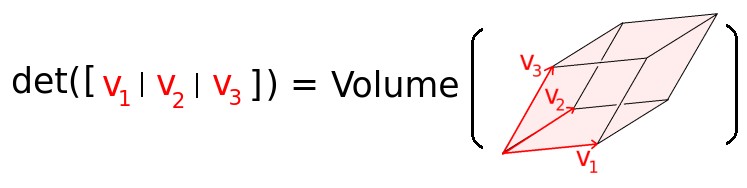
\includegraphics[width=0.6\textwidth]{\main/Images/det0.png}
        \caption{Geometrically, the determinant is equal to the (signed) \textit{hyper}-volume of the parallelepiped spanned by the column (or row) vectors. Here we consider the $d=3$ case, with $A = (\bm{v_1}, \bm{v_2}, \bm{v}_3)^T$.\label{fig:det}}
    \end{subfigure}
    \begin{subfigure}[b]{\textwidth}
        \centering
        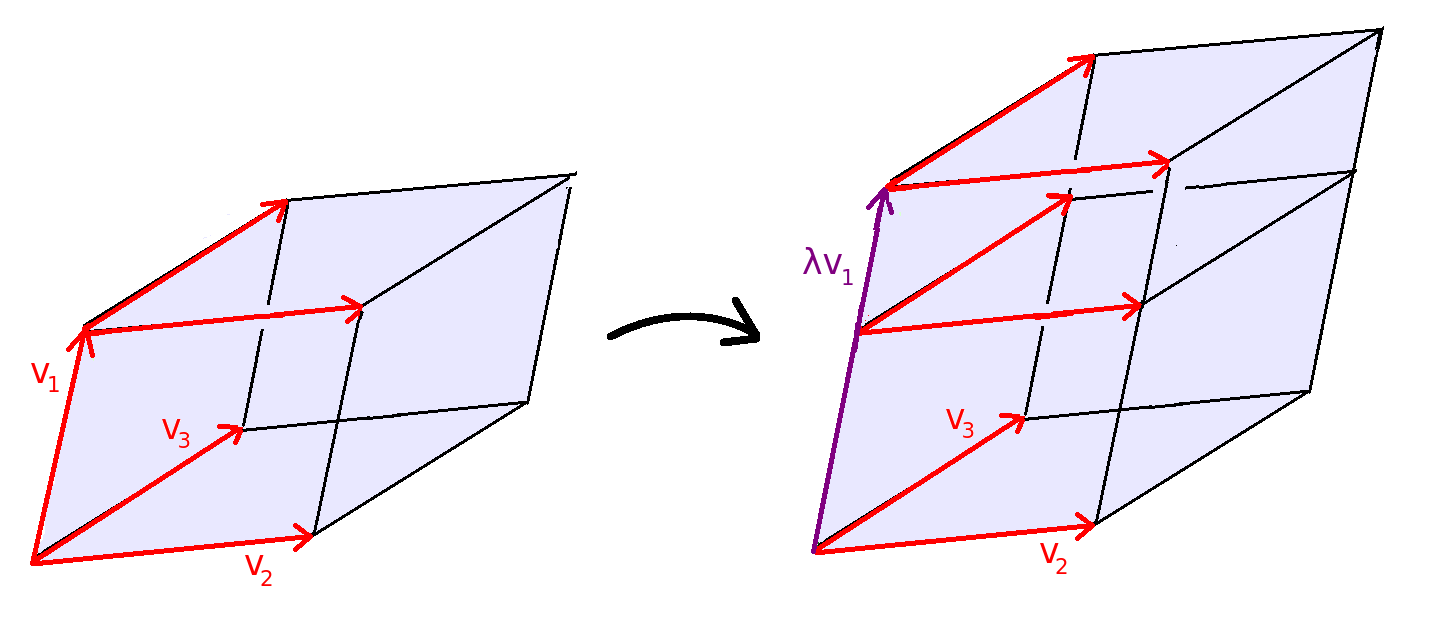
\includegraphics[width=0.6\textwidth]{\main/Images/det1.png}
        \caption{If we scale one of the edges by $\lambda$, the entire volume gets scaled by the same factor $\lambda$. Thus $\operatorname{det}|(\lambda \bm{v_1}, \bm{v_2}, \bm{v_3})^T| = \lambda \operatorname{det}|(\bm{v_1}, \bm{v_2}, \bm{v_3})^T|$}
        \label{fig:scale-det}
    \end{subfigure}
    \\
    \begin{subfigure}[b]{\textwidth}
        \centering
        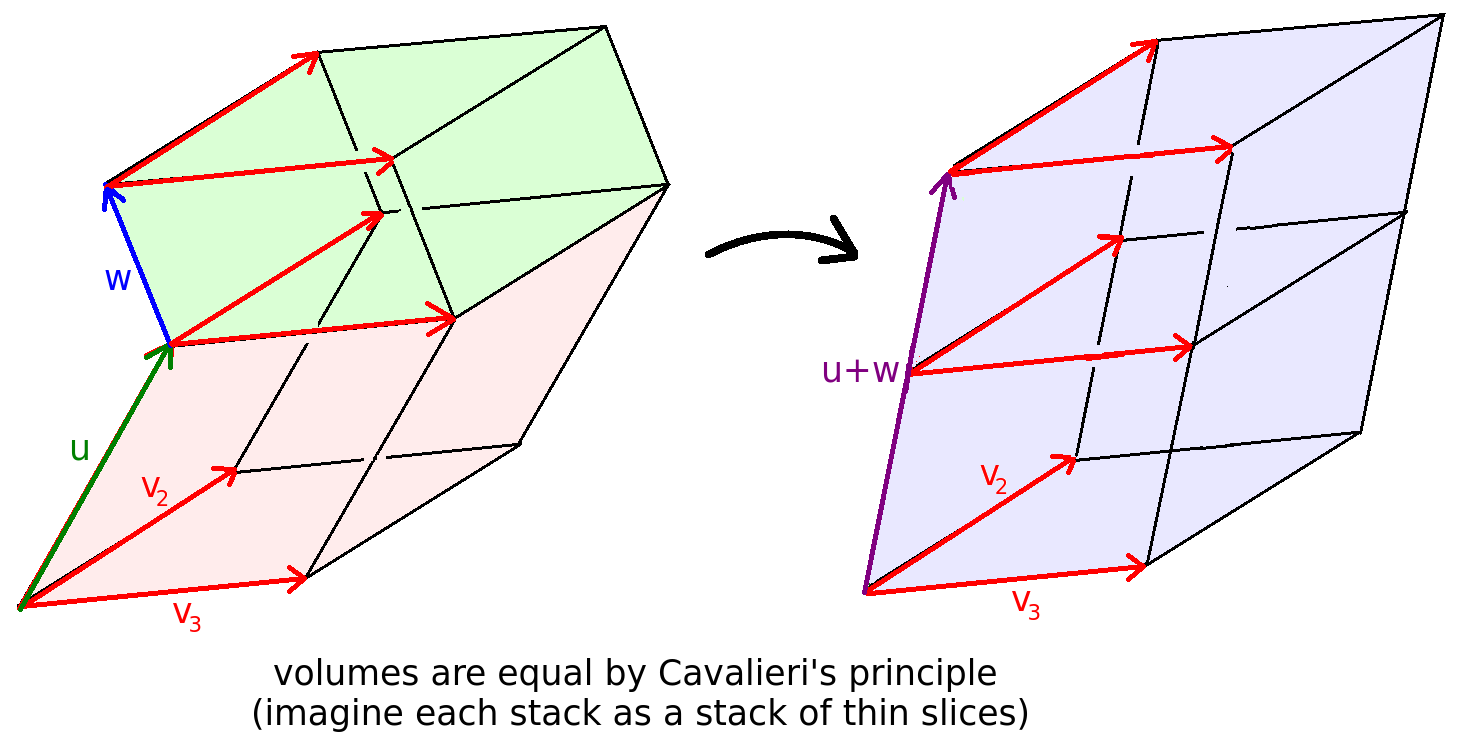
\includegraphics[width=0.6\textwidth]{\main/Images/det2.png}
        \caption{
        The quantity $\operatorname{det}|(\bm{u} + \bm{w}, \bm{v_2}, \bm{v_3})^T|$ is the blue volume on the right, which is equal to the sum of the red volume on the left
($\operatorname{det}|(\bm{u}, \bm{v_2}, \bm{v_3})^T|$) and the green one ($\operatorname{det}|(\bm{w}, \bm{v_2}, \bm{v_3})^T|$), as consequence of Cavalieri's principle. In fact the left figure is obtained from the right one by merely \textit{shifting} some thin slices, which does not change the total volume, as moving around some coins in a stack does not change their number.}
        \label{fig:sum-det}
    \end{subfigure}
       \caption{Geometrical proof of the row/column-linearity of the determinant, taken from \cite{proofdet}.}%
       \label{fig:det-linear}
\end{figure}

\begin{appr}\textbf{Alternative proof for Liouville's theorem} \cite[Chapter~4.1]{sethna}. 

    \medskip

    As particles move in \textit{continuous} trajectories, i.e. they do not \q{teleport} between spatially distant regions, the probability density describing their ensemble must be \textbf{locally conserved}. Mathematically, this means that $\rho(\mathbb{Q}, \mathbb{P})$ satisfies a \textit{continuity equation}:
    \begin{align} \label{eqn:cont-p}
        {\pdv{\rho}{t}} (\mathbb{Q}, \mathbb{P}) = - \grad \cdot \bm{J} (\mathbb{Q}, \mathbb{P}) = - \grad \cdot  [\rho(\mathbb{Q}, \mathbb{P}) \bm{v} (\mathbb{Q},\mathbb{P})]
    \end{align}   
    In other words, the local \textit{change} of $\rho$ over time is equal to the opposite of the \textit{outward flux} $\grad \cdot \bm{J}$ at that point, i.e. the rate of particles traversing a tiny closed surface encompassing $(\mathbb{Q}, \mathbb{P})$ in the outward direction (as consequence of Gauss' theorem). If that flux is positive, then \q{probability is escaping} $(\mathbb{Q}, \mathbb{P})$, and so $\rho$ will decrease. Otherwise, if the outward flux is negative, then \q{probability is gathering} at $(\mathbb{Q}, \mathbb{P})$, and so $\rho$ will rise.

    \medskip

    The flux field $\bm{J}$ is given by $\rho \bm{v}$, where $\bm{v} = (\dot{\mathbb{Q}}, \dot{\mathbb{P}})^T$. So (\ref{eqn:cont-p}) can be rewritten as:
    \begin{align}\nonumber
        \pdv{\rho}{t} &= - \sum_{\alpha=1}^{3N} \left(\pdv{(\rho \dot{q}_\alpha)}{q_\alpha} + \pdv{(\rho \dot{p}_\alpha)}{p_\alpha}\right) = \\
        &= - \sum_{\alpha=1}^{3N} \left(\pdv{\rho}{q_\alpha} \dot{q}_\alpha + \rho \pdv{\dot{q}_\alpha}{q_\alpha}  + \pdv{\rho}{p_\alpha} \dot{p}_\alpha + \rho \pdv{\dot{p}_\alpha}{p_\alpha}\right) \label{eqn:cont-p2}
    \end{align}
    Using Hamilton equations (\ref{eqn:hamilton-eqs}) we can cancel two terms. In fact:
    \begin{align*}
        \pdv{\dot{q}_\alpha}{q_\alpha} \underset{(\ref{eqn:hamilton-eqs})}{=} \pdv{q_\alpha} \pdv{H}{p_\alpha} = \pdv[2]{H}{\textcolor{Red}{q_\alpha}}{\textcolor{Blue}{p_\alpha}} \underset{(a)}{=} \pdv[2]{H}{\textcolor{Blue}{p_\alpha}}{\textcolor{Red}{q_\alpha}} = \pdv{p_\alpha} \pdv{H}{q_\alpha} \underset{(\ref{eqn:hamilton-eqs})}{=} \pdv{p_\alpha} (-\dot{p}_\alpha) = - \pdv{\dot{p}_\alpha}{p_\alpha}
    \end{align*}
    And so (\ref{eqn:cont-p2}) becomes:
    \begin{align*}
        \pdv{\rho}{t} + \sum_{\alpha=1}^{3N} \left( \pdv{\rho}{q_\alpha} \dot{q}_\alpha + \pdv{\rho}{p_\alpha} \dot{p}_\alpha\right) = \dv{\rho}{t} = 0
    \end{align*}
    which is Liouville's theorem.
\end{appr}

\subsection{Consequences of Liouville's theorem}
As system-points flow like an incompressible fluid,\marginpar{Microcanonical ensemble is stationary} a \textit{uniform ensemble} will remain \textit{uniform} indefinitely. Intuitively, a uniform ensemble is just a fluid with a constant definite density. Hamiltonian dynamics just \q{stir} around that fluid, but cannot change its local density anywhere: there cannot be points becoming \q{denser} or \q{more rarefied}. This means that a uniform ensemble (i.e. the \textbf{microcanonical ensemble}) is \textbf{stationary} - and thus is suitable to describe the equilibrium condition. However, at least for now, nothing guarantees that a generic isolate system at equilibrium will reach exactly the stationary state given by the microcanonical. We have proved that it is a \textit{possible solution}, but not \textit{the unique solution}!

\medskip

An other interesting consequence\marginpar{Damping with no attractors} of incompressible flow is that there are no \textbf{attractors}, there are no points in phase space to which many paths \q{converge} over time. So, when we observe a pendulum stopping due to friction in the same place independently of initial conditions, it must not be because it is converging to some definite region of phase-space. Rather, the phase-space paths in which the pendulum loses energy to random air particles are \textit{so much more} than the few where all molecules \q{hit the pendulum at the right times} to keep it going indefinitely.  

\medskip

Liouville's theorem also provides\marginpar{Liouville's theorem and irreversibility} an intuitive explanation for the \textit{second law of thermodynamics}, following an argument by Jaynes \cite{jaynes-secondlaw}\cite{jaynes2}.

Consider a physical system evolving from a macrostate $A$ to another macrostate $B$. If the process $A \to B$ is reproducible, then the volume $W_A$ of microstates compatible with $A$ must \textit{fit} in the volume $W_B$ of microstates compatible with $B$, i.e. $W_A \leq W_B$. In fact, if it were instead $W_A > W_B$, the evolution $A \to B$ would not be reliable: at any $t$, the volume $W_t$ of the evolved ensemble $A(t)$ is the same as $W_A$ (by Liouville's theorem) - and so 
if we require all of $A(t)$ to end up in $B$ (which is necessary for the evolution to happen reliably), then we would be trying to \q{squeeze} too much (incompressible) \q{fluid} $W_A$ in a \q{too small bucket} $W_B$.

\medskip

Entropy in Statistical Mechanics is the logarithm of the volume in phase-space associated with a certain macrostate, and so from $W_A \leq W_B$ follows $S_A \leq S_B$, i.e. the second law of thermodynamics.

\medskip

In the case the inequality holds strictly, then the inverse process $B \to A$ cannot happen reliably. We can estimate the \q{rate of success} of an inverse transition as the ratio $W_A/W_B$. Intuitively, if we try to fill a bucket with $\SI{1}{\l}$ with $\SI{3}{\l}$ of water, only $1$ in $3$ molecules will make it to the end - and the others will be left outside the bucket. Then, we note that even the tiniest difference in entropy would make $W_A/W_B$ negligible, because $S = k_B \ln W$, and so the ratio decays exponentially:
\begin{align*}
    p = \frac{W_A}{W_B} = \exp\left(-\frac{S_B - S_A}{k_B} \right) 
\end{align*}
This means that not only the process $B \to A$ cannot happen reliably, but that it is \textit{so} unreliable that it never happens!

\begin{figure}[H]
    \centering
    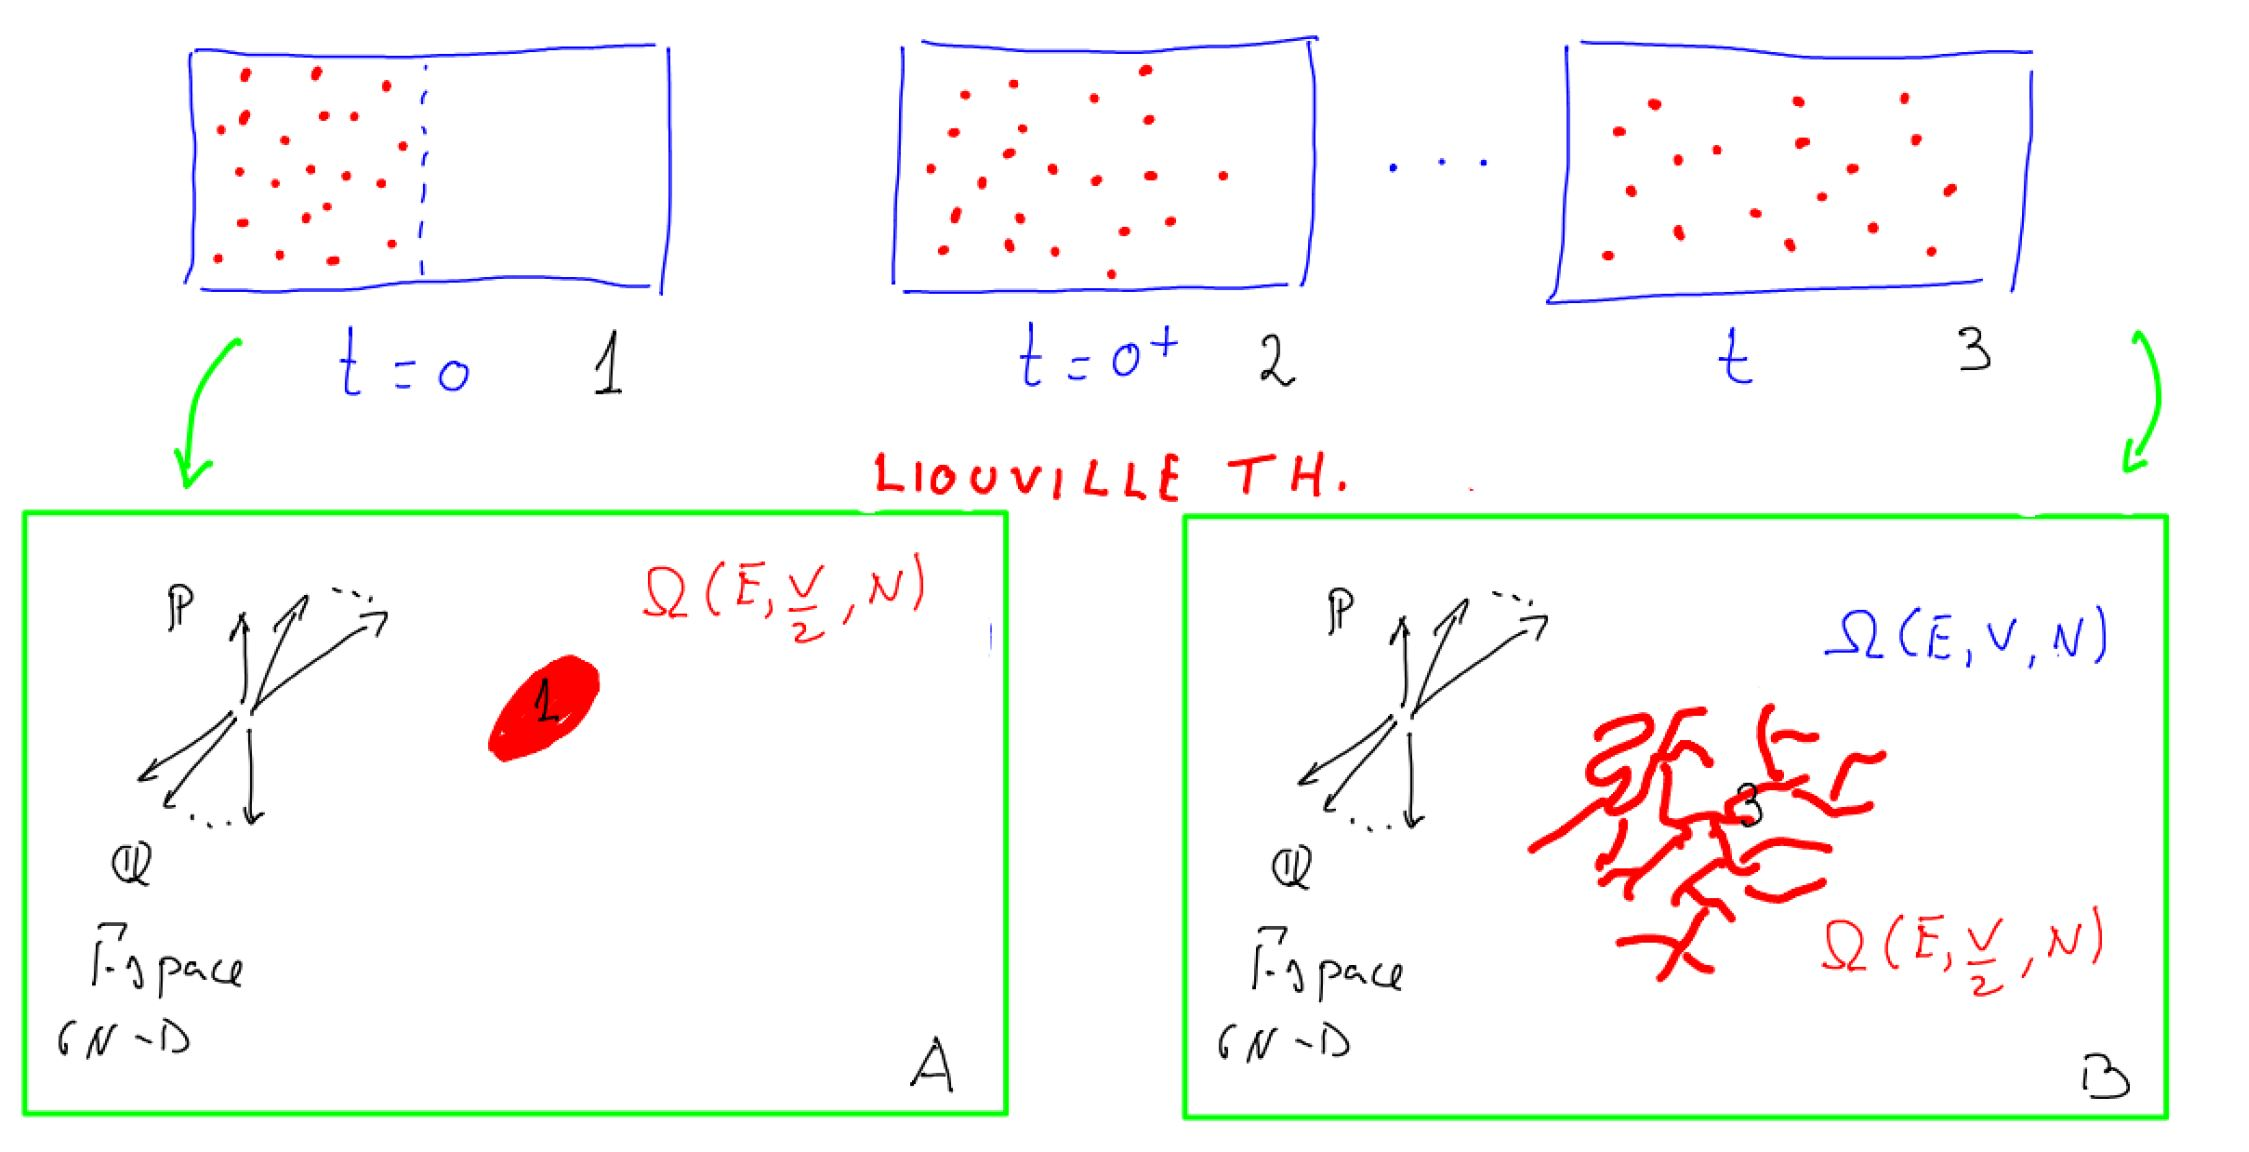
\includegraphics[width=0.93\textwidth]{\main/Images/liouville.png}
    \caption{A gas, initially constrained to the left side of a box (state $A$), is released at $t=0$, and quickly fills the entire volume (state $B$). In phase-space, the ensemble associated with $A$ occupies a volume $\Omega(\mathcal{E}, V/2, N)$, which evolves by \textit{flowing} like an incompressible fluid due to Liouville's theorem. Denote with $A_t$ its evolved version at time $t$, which in general will be \textit{spread} in some complex way. Consider a symmetrized version of $A_t$, obtained by reversing all momenta, and denoted with $\bar{A}_t$. Clearly it has the same volume $\Omega(\mathcal{E}, V/2, N)$ (by symmetry), and if we pick any microstate in it and let it evolve for an interval of time $t$ it will go back to state $A$, because of the reversibility of Hamiltonian mechanics. However, experimentally we have no control on the choice of microstate: when constructing $B$, we effectively pick at random a microstate from a larger set $\Omega(\mathcal{E}, V, N)$, which contains many more paths than the ones coming from $A$ (there is a plethora of ways to obtain a box full of gas). The probability of picking a microstate in $\bar{A}_t$ is given by the ratio $\Omega(\mathcal{E}, V/2, N)/\Omega(\mathcal{E}, V, N) = 2^{-N}$, which is negligible. So, while $A \to B$ happens every time we run the experiment, $B \to A$ is never observed.\\\hspace{\textwidth}
    \textbf{Note}: to be more precise, we should account also for the microstates in $B$ that reach state $A$ in a time $\leq t$, which is a set much larger than the sole $\bar{A}_t$. This makes the discussion much more complex - but the result remains the same.}
    \label{fig:liouville-irreversibility}
\end{figure}

\section{Poincaré Recurrence Theorem}
The \textbf{Poincaré Recurrence Theorem}\index{Theorem!Poincaré Recurrence} states that a mechanical system enclosed in a \textbf{finite volume} and possessing a \textbf{finite} amount of \textbf{energy} will, after a \textit{finite time}, return to an arbitrary small neighborhood of almost any\footnote{Apart from a set of zero measure.} given initial state in phase-space \cite[Chapter~1.7]{mathsm}. In general, the smaller the neighborhood chosen, the larger will be the first arrival time.

\begin{proof}
    Omitted.
\end{proof}

In other words, the Poincaré Recurrence theorem states that everything is \textit{reversible}, given enough time.  
This seems in \textbf{contradiction}  with experience. For example, suppose we start with a gas contained in one half of a box (state $A$), and let it expand freely in the entire box (state $B$). This process is clearly irreversible: the gas will not \textit{spontaneously} return to the initial state. 

If we reverse time, we will obtain a motion $B \to A$ that it is still physically possible, but that in practice never happens. This clearly defines a \textit{preferred direction} for time evolution, a so-called \q{arrow of time}. 

Similarly, if we see a video of an egg crashing on the floor, and that of an egg \q{recomposing} itself after being destroyed, we can surely tell which one has been time-reversed. 

\medskip

%Insert figure
However, Poincaré Recurrence is mathematically proved, and indeed must happen. The key to resolve the apparent contradiction with experience lies in the \textit{amount} of time $T$ required to observe such recurrence. For any macroscopic system, $T$ is orders of magnitude larger than the age of the universe. So, while recurrence \textit{will happen}, it will do so \textit{so far in the future} that it will not matter anymore to anyone!

\medskip

Recurrence can be observed and verified for systems of few particles. For example, consider just $N=2$ particles, moving \textit{at random}\footnote{In classical mechanics, particles follow deterministic trajectories given by Hamilton equations. Here we are implicitly assuming that the resulting motions are comparable with random motion.} in a box. At a given moment, each of them is inside the left half of the box with probability $1/2$. So, the two will be in the left side with probability $1/4$. If we do not care about which side the particles are grouped in, we need to \textit{double} this result: the probability that $N=2$ particles lie in the same side of a box is $1/2$.

\medskip

If we repeat the same computation for $N=3$, we will obtain $p=1/8 \cdot 2 = 1/4$. So, by adding more particles, the \q{grouping probability} quickly decreases, but it is always non-zero. So, given infinite time, the particles will spontaneously return to an half-box configuration an infinite number of times.

\subsection{Heuristic estimate of recurrence time}
To get a sense of the time scales proper of Poincaré recurrence, consider the following heuristic computation.

\medskip

We start with a box filled by $N$ particles of an \textbf{ideal gas}. Let's discretize time, and denote with $X_n$ the \textit{macrostate} of the system at time $t_n$. $X_{n+1}$ depends only on the previous state $X_n$, and so we can model the system as a Markov chain. %What is exactly this state?

If the chain is regular, i.e. if it is possible to start in any state $i$ and reach every other state $j$ given sufficient time, then, due to Kac's lemma (the \textit{basic limit theorem} for Markov chains), the Markov chain will reach, for $t \to \infty$ a \textit{stationary state}, where the probability $\pi_i$ of being in state $i$ is given by:
\begin{align}\label{eqn:kaclemma}
    \pi_i = \frac{1}{\langle T_i \rangle} 
\end{align}
where $T_i$ is the time it takes to visit state $i$ for the first time. 

\medskip

Let $i$ be a macrostate with all particles occupying the left side of the box, corresponding to a region $A_0$ of microstates in phase-space. Then $T_i$ is the time needed for the set of $N$ particles starting on the left side of the box to \textit{regroup} for the first time in the same side.

\medskip

If the deterministic motion is sufficiently chaotic, on the long run it can be considered like if it was random, meaning that all microstates are equiprobable. Then, at stationarity, the probability of the system being in $A_0$ is given by a ratio of phase-space volumes:
\begin{align}\label{eqn:pvmezzo}
    \mathbb{P}(V/2) = \frac{\Omega(\mathcal{E}, V/2, N)}{\Omega(\mathcal{E}, V, N)} = \frac{(V/2)^N \Omega(\mathcal{E},1, N)}{V^N \Omega (\mathcal{E},1,N)} = 2^{-N}
\end{align}
In other words, the microstates with all particles on the left side occupy a phase-space volume of $\Omega_1 \equiv \Omega(\mathcal{E}, V/2, N)$, inside a larger volume of physically possible states $\Omega_2 \equiv \Omega(\mathcal{E}, V, N)$. So, if we pick a microstate at random inside $\Omega_2$, it will be in $\Omega_1$ with probability\footnote{Intuitively, the probability that a coin will drop inside the area of a carpet, is the ratio between the carpet's area and the room's area.} $\Omega_1/\Omega_2$. 

\medskip

Then we take the inverse of the stationary probability to find the number of time step necessary for recurrence. Before doing that, we need to properly specify the size of a single discretized time step. One possibility is to use the characteristic time needed for a gas molecule to visit regions of phase-space sufficiently \q{separated} --- for example the time interval $\tau$ needed to traverse the entirety of the volume. Assuming a square box, the particle needs to travel a length of $V^{1/3}$, and it does so at a mean velocity $\langle |v_x| \rangle$, given by Maxwell's distribution. Then:
\begin{align*}
    \tau \approx \frac{V^{1/3}}{\langle |v_x| \rangle} 
\end{align*}
where:
\begin{align*}
    \langle |v_x| \rangle = \frac{1}{{\int_{\mathbb{R}} \dd{v_x} \exp\left(-\beta m \frac{v_x^2}{2} \right)}}  \int_{\mathbb{R}} \dd{v_x} |v_x| {\exp(-\beta m \frac{v_x^2}{2} )} = \sqrt{\frac{2 k_B T}{\pi m}} = \sqrt{\frac{2 R T}{\pi M_{\mathrm{mol}}} }
\end{align*}
And so the first return time to $i$ is:
\begin{align*}
    \langle T_{\frac{V}{2}} \rangle \underset{(\ref{eqn:kaclemma})}{=} \frac{\tau}{\mathbb{P}(V/2)} \approx \frac{V^{1/3} 2^N}{\langle |v_x| \rangle} 
\end{align*}

Numerically, consider $\SI{1}{\mol}$ of $\rm{O}_2$ ($M_{\mathrm{O}_2} = \SI{32}{\g\per\mol}$), corresponding to $N=N_A = \num{6.2e23}$ molecules in a box of length $V^{1/3} \approx \SI{0.4}{\m}$, at atmospheric pressure $P=\SI{1}{atm}$ and room temperature $T= \SI{300}{\K}$. Then $\langle |v_x| \rangle \approx \SI{500}{\m\per\s}$, and $\langle T_{\frac{V}{2}} \rangle \approx 10^{1.86 \times 10^{23}-11}\,\rm{y}$, which is so much higher than the age of the universe $T_{\mathrm{univ}} = \SI{14e9}{y}$.

\medskip

So, based on this heuristic calculation, we might think that irreversibility is just a matter of \textbf{time scales}: everything is theoretically reversible, but we will never see it reverse any time soon.

\begin{comment}%Moved to following lecture
\subsection{Ergodicity and time averages}

\textbf{Work in progress}

Let $O(\mathbb{Q},\mathbb{P})$ be an observable, and consider its average at time $t$ over the initial conditions:
\begin{align*}
    \langle O(\mathbb{Q}(t), \mathbb{P}(t)) \rangle &= \int_{\bm{\Gamma}} \dd[3N]{\bm{q_0}} \dd[3N]{\bm{p_0}} \rho_0(\mathbb{Q}_0, \mathbb{P}_0) \> O(\mathbb{Q}(t; \mathbb{Q}_0, \mathbb{P}_0), \mathbb{P}(t; \mathbb{Q}_0, \mathbb{P}_0)) =\\
    \shortintertext{We change variables $(\mathbb{Q}(t), \mathbb{P}(t)) \to (\mathbb{Q}, \mathbb{P})$ by introducing two $\delta$\textit{s}:}
    &= \int_{\bm{\Gamma}} \dd[3N]{\bm{q_0}} \dd[3N]{\bm{p_0}} \rho_0(\mathbb{Q}_0, \mathbb{P}_0) \textcolor{Red}{\int_{\bm{\Gamma}} \dd[3N]{\bm{q}} \dd[3N]{\bm{p}} \delta^{3N}(\mathbb{Q}-\mathbb{Q}(t; \mathbb{Q}_0, \mathbb{P}_0)) \delta^{3N}(\mathbb{P} - \mathbb{P}(t; \mathbb{Q}_0, \mathbb{P}_0))} O(\mathbb{Q},\mathbb{P}) =\\
    \shortintertext{In this way we can bring $O(\mathbb{Q}, \mathbb{P})$ outside the inner integral:}
    &= \int_{\bm{\Gamma}} \dd[3N]{\bm{q}} \dd[3N]{\bm{p}} O(\mathbb{Q}, \mathbb{P}) \int_{\bm{\Gamma}} \dd[3N]{\bm{q_0}} \dd[3N]{\bm{p_0}} \rho_0(\mathbb{Q}_0, \mathbb{P}_0) \delta^{3N} (\mathbb{Q}-\mathbb{Q}(t; \mathbb{Q}_0, \mathbb{P}_0)) \> \delta^{3N}(\mathbb{P} - \mathbb{P}(t; \mathbb{Q}_0, \mathbb{P}_0)) =\\
    \shortintertext{And so we have rewritten the average of $O$ in terms of the \textit{evolved} distribution $\rho(\mathbb{Q}, \mathbb{P}, t)$. We want to understand if, in the limit $t \to \infty$, this distribution becomes the one $\rho_{\mathrm{MC}}$ we introduced in the microcanonical ensemble:}
    &\underset{(\ref{eqn:9})}{=}  \int_{\bm{\Gamma}} \dd[3N]{\bm{q}} \dd[3N]{\bm{p}} O(\mathbb{Q}, \mathbb{P}) \rho(\mathbb{Q}, \mathbb{P}, t)  \xrightarrow[t \to \infty]{?} \int_{\bm{\Gamma}} \dd[3N]{\bm{q}} \dd[3N]{\bm{p}} O(\mathbb{Q}, \mathbb{P}) \rho_{\rm{MC}}(\mathbb{Q}, \mathbb{P})  
    \shortintertext{where:}
    \rho_{\rm{MC}} &= \begin{cases}
        \text{const} & \mathcal{E} \leq \mathcal{H}(\mathbb{Q}, \mathbb{P}) \leq \mathcal{E}+ \delta \mathcal{E}\\
        0 & \text{otherwise}
    \end{cases}
\end{align*}


We prepare many systems with different initial conditions distributed according to $\rho_{0}(\mathbb{Q}_0, \mathbb{P}_0)$, evolve each system according to Hamilton equations, compute the value of the observable and then average it.
\end{comment}


%Appr: Jaynes irreversibility with Liouville

\end{document}

